%
% Angepasste FOM Seminarvorlage
%
\documentclass[12pt,a4paper,listof=totoc,bibliography=totoc]{scrartcl}

\usepackage[english]{babel}			% englische Namen/Umlaute
\usepackage[utf8]{inputenc}	    	% Zeichensatzkodierung
\usepackage{silence}
 \WarningFilter{scrartcl}{Usage of package `fancyhdr'}
 \WarningFilter{scrartcl}{Usage of package `parskip'}
\usepackage{fancyhdr}
\usepackage{graphicx}               % Einbinden von Bildern
\usepackage[hidelinks]{hyperref}	% Klickbare Verweise und \autoref{label}
\usepackage[intoc]{nomencl}
\usepackage{setspace}
\usepackage{parskip}
\usepackage{caption}
\usepackage{float}
\usepackage{listings}
\usepackage{scrhack}
\usepackage{geometry}
 \geometry{a4paper, left=40mm, right=20mm, top=40mm, bottom=20mm}
\renewcommand{\familydefault}{\sfdefault}
\renewcommand{\ttdefault}{pcr}
\renewcommand{\lstlistlistingname}{Listings}
\renewcommand{\lstlistingname}{Listing}
\usepackage{float}
\floatstyle{plaintop}
\restylefloat{table}

% Bildueberschrift oben und rechtsbuendig
\captionsetup{labelfont=bf, textfont=bf}
\captionsetup{justification=raggedright,singlelinecheck=false}

% Blocksatz
\def\justify{%
  \rightskip=0pt
  \spaceskip=0pt
  \xspaceskip=0pt
  \relax
}

%
%	Hier werden Titel, Bearbeiter und das Datum eingetragen
%
\newcommand\svthema{NIS2 \& CIS Controls 2}
\newcommand\svperson{Christian Frank (\#473088)}
\newcommand\svdatum{\today}
\newcommand\lvname{Cyber Security Management: Sicherheitsstandards \& Reifegradmodelle}
\newcommand\lvtyp{SS 2025}
\newcommand\lvinst{FOM - Hochschule für Oekonomie \& Management}
\newcommand\lvbetr{Prof. Dr. Jan Hörnemann}

\hypersetup{ % Thema und Author in die Meta-Daten der PDF
  pdftitle={\svthema}, 
  pdfauthor={Christian Frank},
  pdfsubject={Sicherheitsstandards - CIS Benchmarks},
  pdfkeywords={CIS, Benchmarks, NIS2, Security, Kubernetes}
}

\begin{document}

% Titel
\title{ \huge\textbf{\svthema} }
\author{ {\svperson} \\ \svdatum }
\date{ \normalsize \centering 
\includegraphics[width=0.3\textwidth]{FOM}\\ {\lvname} \\ {\lvbetr} \\ {\lvinst} \\ {\lvtyp} }

% Seitennummer oben
\pagestyle{fancy}
\fancyhf{}
\fancyhf[ch]{\thepage}
\renewcommand\headrulewidth{0pt}

\maketitle
\thispagestyle{empty} % laesst die Seitennummer auf der Titelseite verschwinden
\pagenumbering{Roman}

\begin{abstract}
In this paper, we will again examine the NIS2 security standard, review the mappings to the current set of CIS Controls v8.1, and evaluate the use of CSI benchmarks to assess the readiness of Kubernetes clusters for NIS2 and ensure ongoing compliance, thereby mitigating the risks of cyberattacks.

The paper is a continuation of a previous paper that has been revised with new definitions and new aspects of legislation.

\end{abstract}

\vfill
\begin{figure}[h]
    \centering
    
\includegraphics[]{CC-BY}
\end{figure}

This work is licensed under the Creative Commons Attribution 4.0 International License. To view a copy of this license, visit http://creativecommons.org/licenses/by/4.0/ or send a letter to Creative Commons, PO Box 1866, Mountain View, CA 94042, USA.

\cleardoublepage

\tableofcontents			% Inhaltsverzeichnis
\cleardoublepage

\listoffigures				% Abbildungsverzeichnis
\cleardoublepage

\listoftables               % Tabellen
\cleardoublepage

\lstlistoflistings			% Codeverzeichnis
\cleardoublepage

%
% Abkuerzungsverzeichnis
%
\makenomenclature
\renewcommand{\nomname}{List of Abbreviations}

\nomenclature{\textbf{AKS}}{Azure Kubernetes Service}
\nomenclature{\textbf{APA}}{American Psychological Association}
\nomenclature{\textbf{BCM}}{Business Continuity Management}
\nomenclature{\textbf{BIA}}{Business Impact Analysis}
\nomenclature{\textbf{BSI}}{Bundesamt für Sicherheit in der Informationstechnik}
\nomenclature{\textbf{BSIG}}{Gesetz über das BSI}
\nomenclature{\textbf{CIS}}{Center for Internet Security}
\nomenclature{\textbf{CISA}}{Cybersecurity and Infrastructure Security Agency}
\nomenclature{\textbf{CNCF}}{Cloud Native Computing Foundation}
\nomenclature{\textbf{CRA}}{Cyber Resilience Act}
\nomenclature{\textbf{DORA}}{Digital Operational Resilience Act}
\nomenclature{\textbf{ENISA}}{European Union Agency for Cybersecurity}
\nomenclature{\textbf{EU}}{European Union}
\nomenclature{\textbf{EKS}}{Elastic Kubernetes Service}
\nomenclature{\textbf{GKE}}{Google Kubernetes Engine}
\nomenclature{\textbf{IG}}{Implementation Group}
\nomenclature{\textbf{K8s}}{Kubernetes}
\nomenclature{\textbf{NIS}}{Network and Information Security (Directive)}
\nomenclature{\textbf{NIST}}{National Institute of Standards and Technology}
\nomenclature{\textbf{RIA}}{Risk Impact Analysis}
\nomenclature{\textbf{SOC}}{Security Operations Center}

\printnomenclature[1.5in]          % Abkuerzungsverzeichnis
\cleardoublepage

\pagenumbering{arabic}
\setcounter{page}{8}

%
%	Einführung
%

\pagebreak
\section{Introduction}

\onehalfspacing

\subsection{Cyber Security}

Cybersecurity, also called information security or IT security, is the practice of protecting systems, networks, and programs from digital attacks. It aims to reduce the risk of these attacks and prevent the unauthorized exploitation of systems, networks, and technology.

Cybersecurity is an ongoing process because threats and attack vectors are constantly evolving. Organizations and individuals must proactively implement security measures and stay up-to-date on the latest threats.\footnote{See \textit{Gemini (2024)}: What is Cyber Security. \cite{bardCybersec}}

A lot has changed since the first version of the paper, especially regarding the mappings between CIS Controls and NIS2. The changes made it necessary to revisit the experiment and reevaluate the results.\footnote{See \textit{Frank, C. (2024)}: NIS2 and CIS Controls. \cite{previousPaper}}

\subsection{NIS2}

NIS2, which stands for Network and Information Systems Directive II, is the EU's legislative act to strengthen cybersecurity across the European Union. It's essentially an update to the original NIS Directive implemented in 2016.

It sets stricter requirements for various sectors to improve security for essential entities. These entities include organizations in critical sectors like energy, transport, waste management, healthcare, and digital infrastructure providers.\footnote{See \textit{NIS 2 Compliant.org (2024)}: Comprehensive Guide to the NIS 2 Directive. \cite{nisGuide}}

Compared to the original directive, NIS2 applies to a broader range of businesses and organizations; it recognizes the importance of securing the supply chain and includes measures to address vulnerabilities in third-party vendors and suppliers.

It also emphasizes a risk-based approach to cybersecurity. Organizations must identify and assess their security risks and implement appropriate mitigation measures. Classical tools from Business Continuity Management, such as Risk Impact Analysis and Business Impact Analysis, are now essential parts of the cybersecurity toolkit.\footnote{See \textit{BSI (2025)}: Business Impact Analysis. \cite{bsiBCM}}

NIS2 entered into force on 16 January 2023, and the Member States had 21 months, until 17 October 2024, to transpose its measures into national law.\footnote{See \textit{Negreiro-Achiaga, M. (2023)}: The NIS2 Directive. \cite{nisBrief}}

As of the time of writing, the German government has just presented a proposal to the legislature to codify NIS2 into national law.\footnote{See \textit{BSI (2025)}: NIS-2-Regierungsentwurf. \cite{presseNis2}}

\subsection{CIS Controls and Benchmarks}

CIS Controls, or CIS Critical Security Controls, are a prioritized set of best practices designed to improve an organization's cybersecurity posture. Developed by the \href{https://www.cisecurity.org/}{Center for Internet Security} (CIS), a non-profit organization, these controls are a widely trusted framework for defending against cyberattacks.\footnote{See \textit{CIS (2024)}: Critical Security Controls. \cite{cisControls}}

CIS Benchmarks are configuration guides intended to harden various IT systems against cyberattacks based on the CIS' Critical Security Controls. They provide a set of best practices for securing specific operating systems, applications, and cloud platforms. Many of these Benchmarks have specific versions tied to the underlying software version.\footnote{See \textit{CIS (2024)}: CIS Benchmarks List. \cite{cisBenchmarks}}

Most Kubernetes platform vendors provide automated tools to check against these benchmarks and report and enforce compliance as a first line of defense.

\subsection{Kubernetes}

Kubernetes, or K8s, is an open-source system designed to automate deploying, scaling, and managing applications built using containers. Containers package software in a standardized unit that includes all dependencies the software needs to run, like code, libraries, and settings. This makes them portable and efficient.

Kubernetes helps manage these containers by grouping them logically. This makes it easier to track and manage complex applications with many containers. The original inspiration for Kubernetes came from Google's internal container orchestration system, Borg.\footnote{See \textit{Gemini (2024)}: What is Kubernetes. \cite{bardKubernetes}} 

In 2015, Kubernetes reached the 1.0 milestone, and in 2016, it was donated to the CNCF; the current release of Kubernetes is 1.33, codenamed Octarine. The cutest release was 1.30, codenamed Uwubernetes.

"For the people who built it, for the people who release it, and for the furries who keep all of our clusters online, we present to you Kubernetes v1.30: Uwubernetes, the cutest release to date."\footnote{\textit{Dsouza, A. (2024)}: Kubernetes 1.30. \cite{uwubernetes}}

\begin{figure}[H]
\centering
\caption {Kubernetes 1.30 Release Logo}

\includegraphics[width=0.3\linewidth]{images/k8s-1.30.png}
\label{fig:uwubernetes}
\end{figure}

\subsection{Research Question \& Method}

This paper will examine the new NIS2 security standards, compare them to the current CIS v8 controls, and attempt to map them with a focus on using the CSI Benchmarks. Once we've established a helpful relationship, we will evaluate using CSI benchmarks to check Kubernetes clusters for NIS2 compliance. We will also check whether CIS Benchmarks can provide information about the level of compliance for Kubernetes clusters and offer actionable insights into reaching NIS2 compliance for the relevant controls.

To do this, we will perform an Experiment and check the findings of the Kubernetes CIS Benchmarks on a random cluster.\footnote{See \textit{Genau, L. (2020)}: Ein Experiment in deiner Abschlussarbeit durchführen. \cite{expScribbr}}

The goal of this paper is to determine if CIS Kubernetes Benchmark results can indicate whether a Kubernetes cluster is NIS2-compliant on the platform level.

\subsection{Gender-neutral Pronouns}

Our society is becoming more open, inclusive, and gender-fluid, and now I think it's time to think about using gender-neutral pronouns in scientific texts, too. Two well-known researchers, Abigail C. Saguy and Juliet A. Williams, both from UCLA, propose to use the singular they/them instead: "The universal singular they is inclusive of people who identify as male, female, or nonbinary."\footnote{\textit{Saguy, A. (2020)}: Why We Should All Use They/Them Pronouns. \cite{pronouns}} The aim is to support an inclusive approach in science through gender-neutral language. 

In this paper, I'll attempt to follow this suggestion and invite all my readers to do the same for future articles. Thank you!

If you're not sure about the definitions of gender and sex and how to use them, have a look at the definitions by the American Psychological Association.\footnote{See \textit{APA (2021)}: Definitions Related to Sexual Orientation. \cite{apaDefinitions}}

\subsection{Climate Emergency}

As Professor Rahmstorf puts it: "Without immediate, decisive climate protection measures, my children currently attending high school could already experience a 3-degree warmer Earth. No one can say exactly what this world would look like—it would be too far outside the entire experience of human history. But almost certainly, this earth would be full of horrors for the people who would have to experience it."\footnote{\textit{Rahmstorf, A. (2024)}: Climate and Weather at 3 Degrees More. \cite{3dgreesMore}}


%
%	Begrifflichkeiten
%

\pagebreak
\section{NIS2 \& CIS}

\onehalfspacing

\subsection{The Network and Information Security Directive}

The European Commission and the High Representative of the Union for Foreign Affairs and Security Policy presented a new EU Cybersecurity Strategy at the end of 2020, the second version of the Network and Information Security Directive (NIS2).\footnote{See \textit{EU (2023)}: Cybersecurity Policies. \cite{cyberPol}}

We will first examine some key components introduced with the directive and then compare this to an already established industry framework.

\subsubsection{EU Cybersecurity Agency ENISA}

The European Union Agency for Cybersecurity (ENISA) is a key player in ensuring high cybersecurity across Europe. Established in 2004 and empowered by the EU Cybersecurity Act, ENISA contributes to EU cyber policy, promotes trustworthy Information and Communications Technology products and services, collaborates with Member States and EU bodies, and prepares Europe for future cyber threats. By sharing knowledge, building capacity, and raising awareness, ENISA works with stakeholders to strengthen trust in the connected economy, boost resilience, and safeguard Europe's society and citizens in the digital age.\footnote{See \textit{EU (2024)}: About Enisa. \cite{aboutEnisa}}

\subsubsection{EU Cybersecurity Act}

The EU Cybersecurity Act is the central legislation strengthening the EU's cybersecurity capabilities. It enhances the role of ENISA, the EU Agency for Cybersecurity, and establishes a robust certification framework for products and services.

Key provisions of the EU Cybersecurity Act:

\begin{itemize}
    \item Strengthened ENISA: The Act grants ENISA a permanent mandate, increases its resources, and assigns it new responsibilities.
    \item Certification framework: ENISA will play a pivotal role in establishing and maintaining a European cybersecurity certification framework.
    \item Public information: ENISA will provide information on certification schemes and issued certificates through a dedicated website.
    \item Operational cooperation: ENISA will facilitate cooperation between EU Member States in handling cybersecurity incidents and coordinating responses to large-scale cross-border attacks.\footnote{See \textit{EU (2023)}: The EU Cyber Security Act. \cite{cyberSec}}
\end{itemize}

\subsubsection{EU Cyber Resilience Act}

The Cyber Resilience Act (CRA) is a significant step towards safeguarding consumers and businesses from cybersecurity vulnerabilities. By introducing mandatory cybersecurity requirements for manufacturers and retailers, the CRA addresses the issue of inadequate security features in products and software. It also aims to empower consumers and businesses by providing them with clear information about the cybersecurity of products and ensuring that they are designed and maintained with security in mind. The CRA's key benefits include:

\begin{itemize}
    \item Harmonized rules: Consistent rules for products with a digital component.
    \item Cybersecurity framework: Requirements for planning, design, development, and maintenance of products.
    \item Duty of care: Obligation to ensure product security throughout its lifecycle.
    \item Consumer protection: Improved ability for consumers to make informed choices.
    \item Business security: Enhanced protection for businesses using digital products.\footnote{See \textit{EU (2024)}: Cyber Resiliency Act. \cite{cyberResiliency}}
\end{itemize}

\subsubsection{EU Cyber Solidarity Act}

The Act seeks to improve preparedness, detection, and response to significant cybersecurity threats by establishing a European Cybersecurity Alert System and a comprehensive Cybersecurity Emergency Mechanism.

Key features of the EU Cyber Solidarity Act:

\begin{itemize}
    \item European Cybersecurity Alert System: This system will consist of interconnected Security Operation Centers (SOCs) across the EU, using advanced technologies like AI and data analytics to detect and share threat warnings.
    \item Cybersecurity Emergency Mechanism: This mechanism will provide a framework for coordinated responses to large-scale cyberattacks and crises.
    \item Enhanced capacities: The Act will strengthen the EU's capacity to detect, prepare for, and respond to cybersecurity incidents.
\end{itemize}

The European Cybersecurity Shield, a component of the Act, is a pilot initiative involving three cross-border Security Operations Center consortia. Launched in November 2022, this pilot project aims to test and refine the concept of a networked system of SOCs for early threat detection and sharing.\footnote{See \textit{EU (2024)}: Cyber Solidarity Act. \cite{cyberSol}}

\subsubsection{EU Certification Framework}

The EU Cybersecurity Act provides the foundation for establishing an EU-wide cybersecurity certification framework, with ENISA playing a central role in its development and implementation. This framework will offer a standardized approach to assessing the cybersecurity of products and services, enhancing consumer confidence, and protecting businesses from cyber threats.

At the time of writing, there is no official certification program yet.

\subsection{Center for Internet Security}

All the institutions mentioned above are part of the EU's attempt to provide a legal and regulatory framework for cyber security. However, several established frameworks are already available within the private sector, one of which is CISecurity.

CISecurity is an acronym for the Center for Internet Security. It's a non-profit organization that helps individuals, businesses, and governments protect themselves from cyber threats. Their key offerings are CIS Controls and CIS Benchmarks.

The Center for Internet Security was founded 20 years ago in Washington, D.C., in response to increased cyber-attacks. It has established itself as the go-to resource for computer security, but unlike ENISA, CISecurity is not a government organization.

Its funding comes from various government and non-profit grant programs designed to improve the overall cybersecurity posture of the U.S. and through the sale of various cybersecurity best practices tools and resources, such as CIS SecureSuite Membership and CIS Hardened Images, and cybersecurity services like CIS Endpoint Security Services.

\subsubsection{CIS Controls}

CIS Controls are actionable and prioritized recommendations that provide organizations with a cybersecurity defense strategy and improve their cybersecurity posture.\footnote{See \textit{CIS (2024)}: Critical Security Controls. \cite{cisControls}}

CIS Controls are organized into Implementation Groups:

\begin{itemize}
    \item IG1 is a minimum standard of information security aimed at all enterprises.
    \item IG2 focuses on enterprises dealing with sensitive client or company information.
    \item IG3 focuses on the impact of zero-day attacks and targeted attacks from sophisticated adversaries and might not be suitable for all enterprises.
\end{itemize}

Implementation groups are cumulative; i.e., to implement IG2, you would also need to implement IG1.

The CIS Controls are a standalone toolset. There are mappings available for other security and compliance requirements, such as ISO 27001, NIST CSF, or NIST SP 800-53.\footnote{See \textit{CIS (2024)}: Critical Controls Mappings. \cite{cisMappings}}

At the time of writing, an official mapping to NIS2 is not yet available but will hopefully emerge soon.

\subsubsection{CIS Benchmarks}

CIS Benchmarks are detailed configuration guidelines for operating systems, hardware, and software. These can be validated and monitored automatically using specialized tools.

The Benchmark itself addresses the CIS Controls safeguards of Secure
Configurations and maintaining a Secure Configuration Process without individual mappings to these safeguards.\footnote{See \textit{CIS (2024)}: Benchmark List. \cite{cisBenchmarks}}

In CIS Controls v8, this would be Control 4.1, "Establish and Maintain a Secure Configuration Process"; in CIS Controls v7, it was Control 5.1, "Establish Secure Configurations." Both Controls are part of the Implementation Group IG1 in their respective version.

The CIS Benchmarks do not address other controls.\footnote{See \textit{CIS (2024)}: CIS Critical Security Controls FAQ. \cite{cisFaq}} For the remainder of this paper, we will focus on the CIS Benchmarks applicable to Kubernetes and the CIS Controls that can be monitored through CIS Benchmarks and link these to the NIS2 Directive.

\subsection{CIS Benchmarks on Kubernetes}

To easily manage the security of a set of Kubernetes clusters, we can turn to Rancher.

What is Rancher? The Rancher Labs website states it is "[...] a complete software stack for teams adopting containers. It addresses the operational and security challenges of managing multiple Kubernetes clusters while providing DevOps teams with integrated tools for running containerized workloads."\footnote{\textit{Rancher Labs (2019)}: Run Kubernetes Everywhere. \cite{rancher}}

Using a user-friendly GUI, Rancher provides a management platform to centrally manage multiple Kubernetes clusters in Enterprise IT. It also offers application development integration tools and robust enterprise-grade security and governance features. For operations, Rancher provides integrated solutions for logging, monitoring, and auditing, together with many other features, such as CIS scans or a built-in service mesh.

The classic Rancher GUI looks like this:

\begin{figure}[H]
\centering
\caption {Rancher Dashboard}
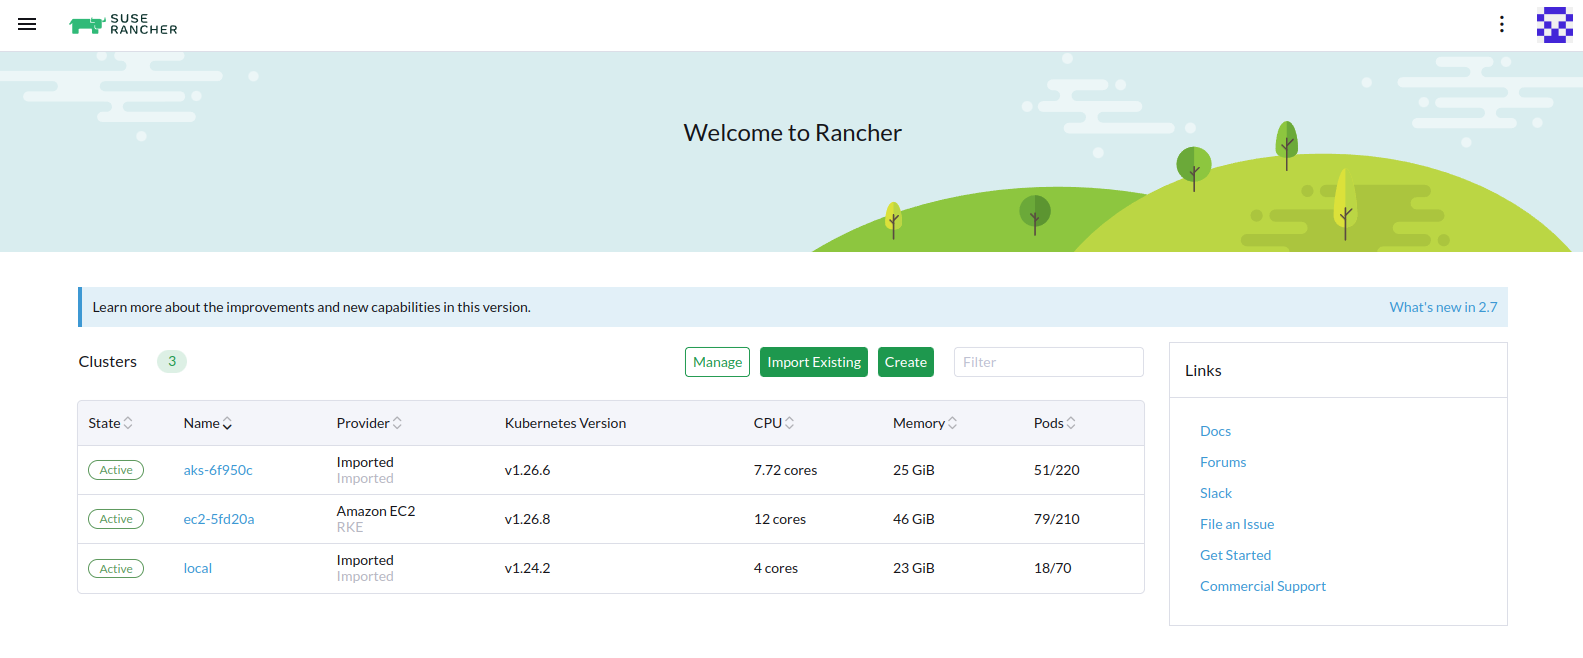
\includegraphics[width=\linewidth]{images/rancher-dashboard.png}
\label{fig:rancherDashboard}
\end{figure}

This paper will use Rancher's integrated CIS benchmarks for further analysis.

\subsubsection{Cluster Management Tools}

CIS Scans are one of the available cluster management applications within Rancher.

The Rancher CIS Benchmark uses \href{https://github.com/aquasecurity/kube-bench}{kube-bench}, an open-source tool from \href{https://www.aquasec.com/}{Aqua Security}, to check clusters for CIS Kubernetes Benchmark compliance. To generate a cluster-wide report, the application utilizes \href{https://sonobuoy.io/}{Sonobuoy} for report aggregation.\footnote{See \textit{Rancher Labs (2024)}: CIS Scans. \cite{rancherBenchmarks}}

Rancher includes many Benchmark profiles to support the various supported versions of downstream Kubernetes clusters.

\subsubsection{CIS Scans Installation}

CIS Benchmarks can be installed within the Rancher UI as a Cluster Management application or using Infrastructure-as-Code automation, e.g., \href{https://www.terraform.io/}{Terraform}.

\begin{lstlisting}[caption=Installing CIS Benchmarks, frame=single, basicstyle=\ttfamily]
# CIS Benchmarks
resource "rancher2_app_v2" "cisbench_fom" {
  lifecycle {
    ignore_changes = all
  }
  cluster_id = rancher2_cluster.cluster_fom.id
  name = "rancher-cis-benchmark"
  namespace = "cis-operator-system"
  project_id = data.rancher2_project.system.id
  repo_name = "rancher-charts"
  chart_name = "rancher-cis-benchmark"
  chart_version = var.cischart
}
\end{lstlisting}

\subsubsection{CIS Scans Reports}

After installation, the CIS Benchmarks are available within the GUI for manual or scheduled executions, in this case, for an Azure Kubernetes Service downstream Kubernetes cluster.

\begin{figure}[H]
\centering
\caption {CIS Scans}
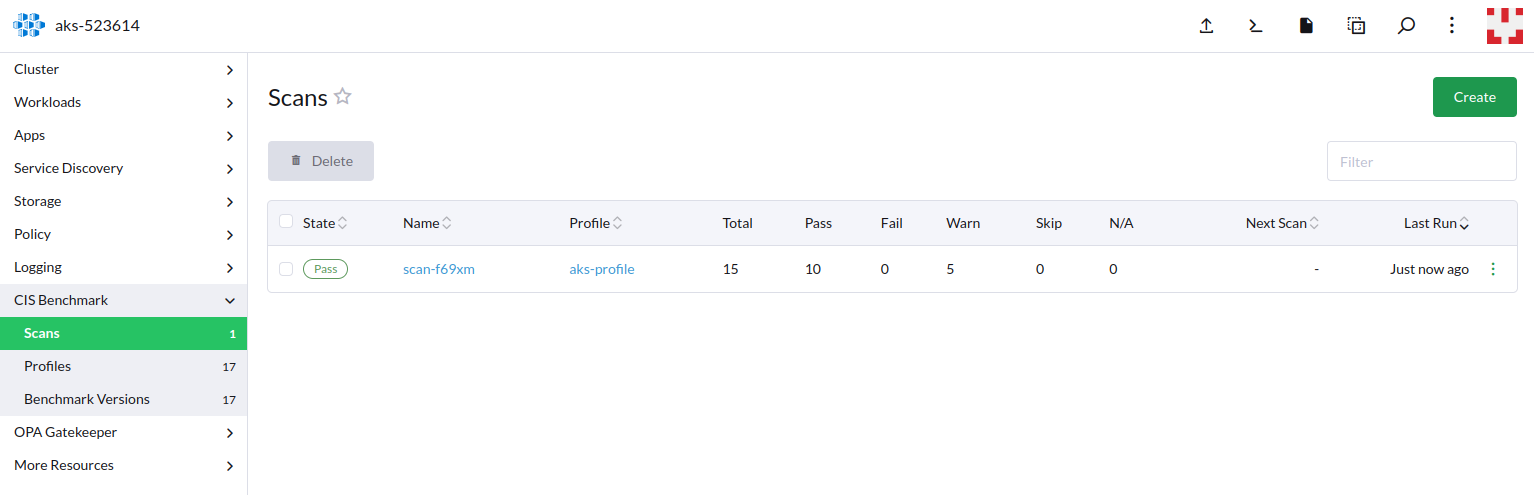
\includegraphics[width=\linewidth]{images/cis-scans-1.png}
\label{fig:cisScans}
\end{figure}

After a scan, the results will also be available in the GUI.

\begin{figure}[H]
\centering
\caption {CIS Scans Results AKS}
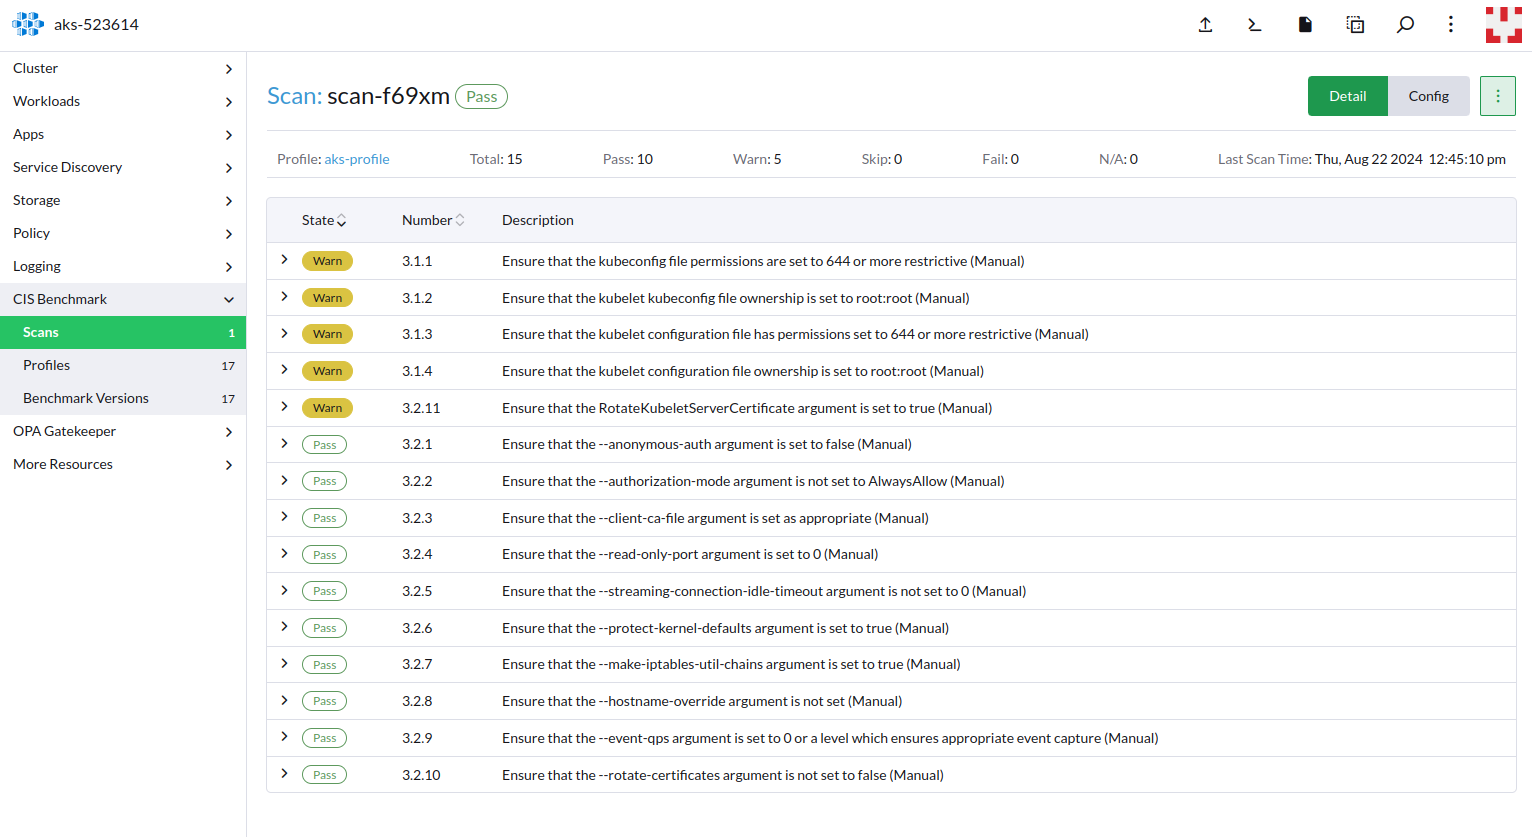
\includegraphics[width=\linewidth]{images/cis-scans-2.png}
\label{fig:cisAKS}
\end{figure}


%
%	Theorieteil
%

\pagebreak
\section{NIS2 Exploration}

\onehalfspacing

\subsection{Mapping between NIS2 and CIS Controls 8.1}

\subsection{Mapping between NIST SP 800-53 and CIS Controls 8.1}

\subsection{Mapping between NIST SP 800-171 and CIS Controls 8.1}

\subsection{NIS2 Article 21}

The NIS2 directive itself is a legal document organized into Chapters and Articles. It has a pan-European scope and targets critical businesses. NIS2 applies to many entities that provide essential services to the European economy and society, such as Operators of Essential Services (OES) and Digital Service Providers (DSPs). While NIS2 primarily targets medium and large enterprises, smaller entities may still be affected, depending on the services they provide.

As we've seen, much of the content concerns reporting requirements and EU-wide cooperation and institutions, which we will not analyze further in this paper.\footnote{See \textit{EU (2022)}: NIS2 Directive. \cite{nis2}}

Article 21, however, defines the required Cybersecurity risk-management measures for critical infrastructure. In paragraph 2, point (g), NIS2 calls for basic cyber hygiene practices and cybersecurity training.

Any entity covered by the directive must, thus, have an IT Security Policy to implement basic cyber hygiene.\footnote{See \textit{NIS 2 Compliant.org (2024)}: List of Policies Required by NIS 2 Directive. \cite{nisPols}} To strengthen their security postures, entities could rely on one of the major frameworks and standards, such as the NIST SP 800 series, ISO/IEC 27001, Mitre Att\&ck, or CIS Controls.\footnote{See \textit{NIS 2 Compliant.org (2024)}: Requirements Checklist for NIS 2. \cite{nisReqs}}

The directive does not mandate whether an entity chooses one of these frameworks or creates its own policies. It also does not favor or champion any of the mentioned frameworks.

For this paper, we will focus on CIS Controls and the baselines provided by the CIS Benchmarks to fulfill Article 21's requirements.

\subsection{CIS Control 04}

The CIS Controls in the current version (v8) consist of 18 controls:

\begin{enumerate}
    \item Inventory and Control of Enterprise Assets
    \item Inventory and Control of Software Assets
    \item Data Protection
    \item Secure Configuration of Enterprise Assets and Software
    \item Account Management
    \item Access Control Management
    \item Continuous Vulnerability
    \item Audit Log Management
    \item Email and Web Browser Protections
    \item Malware Defenses
    \item Data
    \item Network Infrastructure
    \item Network Monitoring and Defense
    \item Security Awareness and Skills Training
    \item Service Provider
    \item Application Software Security
    \item Incident Response
    \item Penetration Testing\footnote{See \textit{CIS (2024)}: Critical Security Controls v8. \cite{cisControls}}
\end{enumerate}

As with the NIS2 articles, many of these controls are procedural and cannot be automated. Control 04, however, Secure Configuration of Enterprise Assets and Software, is of particular importance for individual IT systems, such as Kubernetes clusters.

Control 04 consists of several subcontrols:

\begin{enumerate}
    \item Establish and Maintain a Secure Configuration Process
    \item Establish and Maintain a Secure Configuration Process for
Network Infrastructure
    \item Configure Automatic Session Locking on Enterprise Assets
    \item Implement and Manage a Firewall on Servers
    \item Implement and Manage a Firewall on End-User Devices
    \item Securely Manage Enterprise Assets and Software
    \item Manage Default Accounts on Enterprise Assets and Software
    \item Uninstall or Disable Unnecessary Services on Enterprise Assets
and Software
    \item Configure Trusted DNS Servers on Enterprise Assets
    \item Enforce Automatic Device Lockout on Portable End-User Devices
    \item Enforce Remote Wipe Capability on Portable End-User Devices
    \item Separate Enterprise Workspaces on Mobile End-User Devices\footnote{See \textit{CIS (2024)}: Critical Security Controls v8 - Control 04. \cite{cisControls}}
\end{enumerate}

Control 4.1 strongly emphasizes the configuration process, as the default configuration for enterprise software is typically geared toward ease of deployment and use rather than security. This is where the CIS Benchmarks come into play.

\subsection{NIS2 Article 21 and CIS Control 04}

Control 4.1 is the prime candidate to support and evaluate NIS2 Article 21 2(g) as it covers basic cyber hygiene and IT security policy.

The requirements in Article 21 are much broader than those of CIS Control 04, but a secure configuration process is a fundamental element.

Fulfilling CIS Control 04 does not imply compliance with Article 21, but noncompliance with CIS Control 04 does imply noncompliance with Article 21.

The CIS Benchmarks can indicate whether an IT system is potentially NIS2 compliant. Evaluating and running the CIS Benchmarks regularly will support NIS2 compliance checking and defense against cyber attacks.

\subsection{CIS Benchmarks on AKS}

Maintaining a Secure Configuration Process is important. Leaving default configurations unchecked might result in some of these security risks:

\begin{itemize}
    \item Exposed Services and Ports
    \item Default Accounts and Passwords
    \item Pre-configured DNS Settings
    \item Older or Vulnerable Protocols
    \item Pre-installed Unnecessary Software\footnote{See \textit{CIS (2024)}: Ibid. \cite{cisControls}}
\end{itemize}

To mitigate these, the CIS Benchmarks provide a security baseline for enterprise software, such as Kubernetes, covering all aspects of CIS Control 4.1 and a matching IT Security Policy.\footnote{See \textit{CIS (2024)}: CIS Benchmarks List. \cite{cisBenchmarks}}

There are CIS Benchmarks tailored to the currently available and supported version of Kubernetes and the major hosted versions, such as the Azure Kubernetes Engine.

\subsection{CIS Benchmarks on RKE2}

\subsection{CIS Kubernetes Benchmark Results}

We'll use the Rancher CIS Scans from above against a simple downstream RKE2 Kubernetes cluster; the Kubernetes Version is v1.28.12+rke2r1, and the CIS Scans application version is v5.3.0.

Running CIS profile 1.8 against our cluster, we receive the following results:

\begin{figure}[H]
\centering
\caption {CIS Scans Results RKE2}
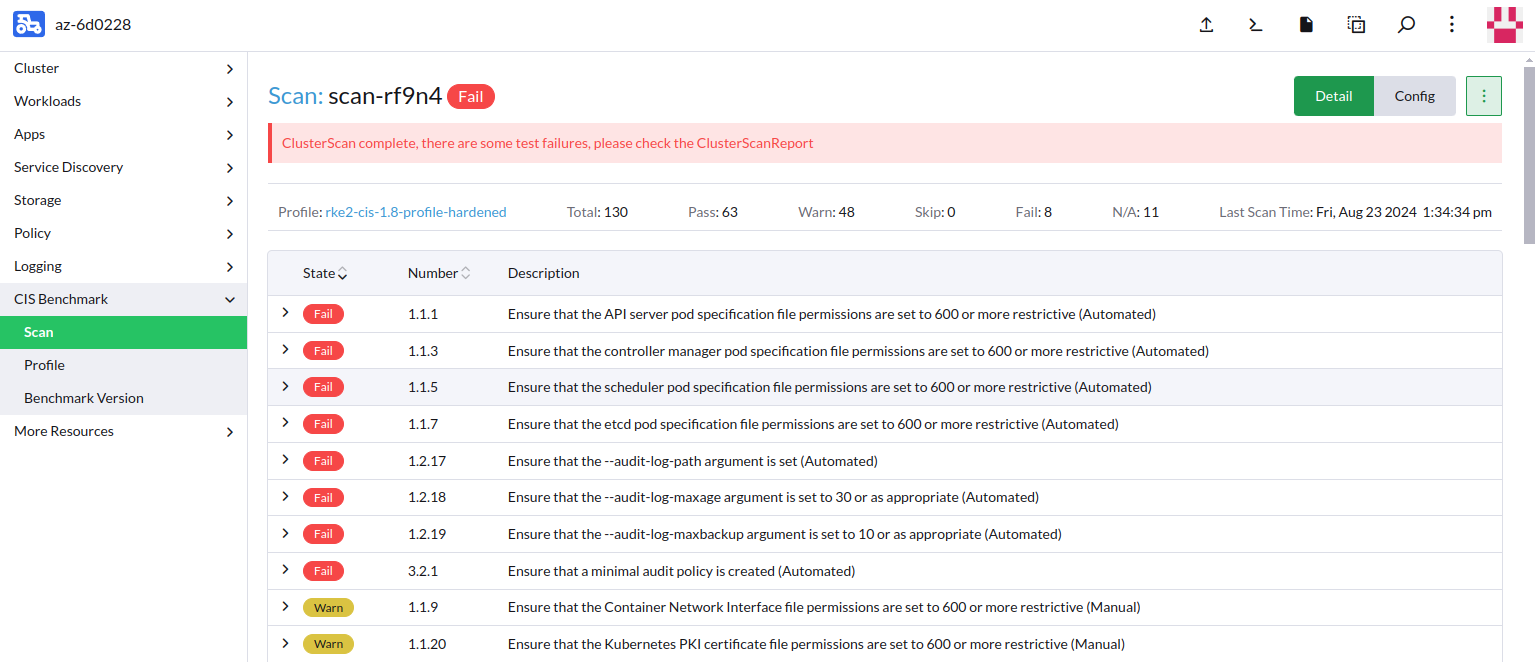
\includegraphics[width=\linewidth]{images/cis-scans-3.png}
\label{fig:cisRKE2}
\end{figure}

Compared to the results from an AKS downstream cluster above, we can see that there are many more failures and warnings. The difference between these two types of clusters, even though they are both Kubernetes v1.28 clusters, is that AKS is a hosted version of Kubernetes. In a hosted version of Kubernetes, the hosting entity provides the control plane, in this case, Microsoft Azure. An RKE2 cluster, however, does include the Kubernetes control plane and thus has a much higher attack surface and many more configuration options.

In the next chapter, we will look at some failures and warnings and possible mitigation steps.


%
%	Praxisbezug
%

\pagebreak
\section{NIS2 Analysis}

\onehalfspacing

\subsection{Running the CIS Benchmarks}

To examine the results of a CIS Benchmark, we will create a Kubernetes cluster on Microsoft Azure with the following versions:

\begin{itemize}
    \item Microsoft AKS v1.32
    \item CIS AKS Benchmark v1.7
    \item kube-bench v0.11.2
    \item SUSE Rancher v2.11.3
    \item Terraform v1.12
\end{itemize}

We will create the cluster with a default node pool and without hardening to get reproducible results that will be relevant for most environments:

\begin{lstlisting}[caption=Terraform Plan, frame=single, basicstyle=\ttfamily]
# AKS cluster
resource "azurerm_kubernetes_cluster" "cluster_az" {
  name                = "aks-${random_id.instance_id.hex}"
  location            = var.az-region
  resource_group_name = var.az-resource-group
  kubernetes_version  = var.k8version
  dns_prefix          = "aks-${random_id.instance_id.hex}"
  web_app_routing {
    dns_zone_ids = []
  }
  local_account_disabled = "false"
  default_node_pool {
    name       = "agent${random_id.instance_id.hex}"
    node_count = var.numnodes
    vm_size    = var.type
  }
  identity {
    type = "SystemAssigned"
  }
}            
\end{lstlisting}
This is the resulting AKS cluster that we will use for our test:

\begin{figure}[H]
\centering
\caption {AKS Cluster Dashboard}
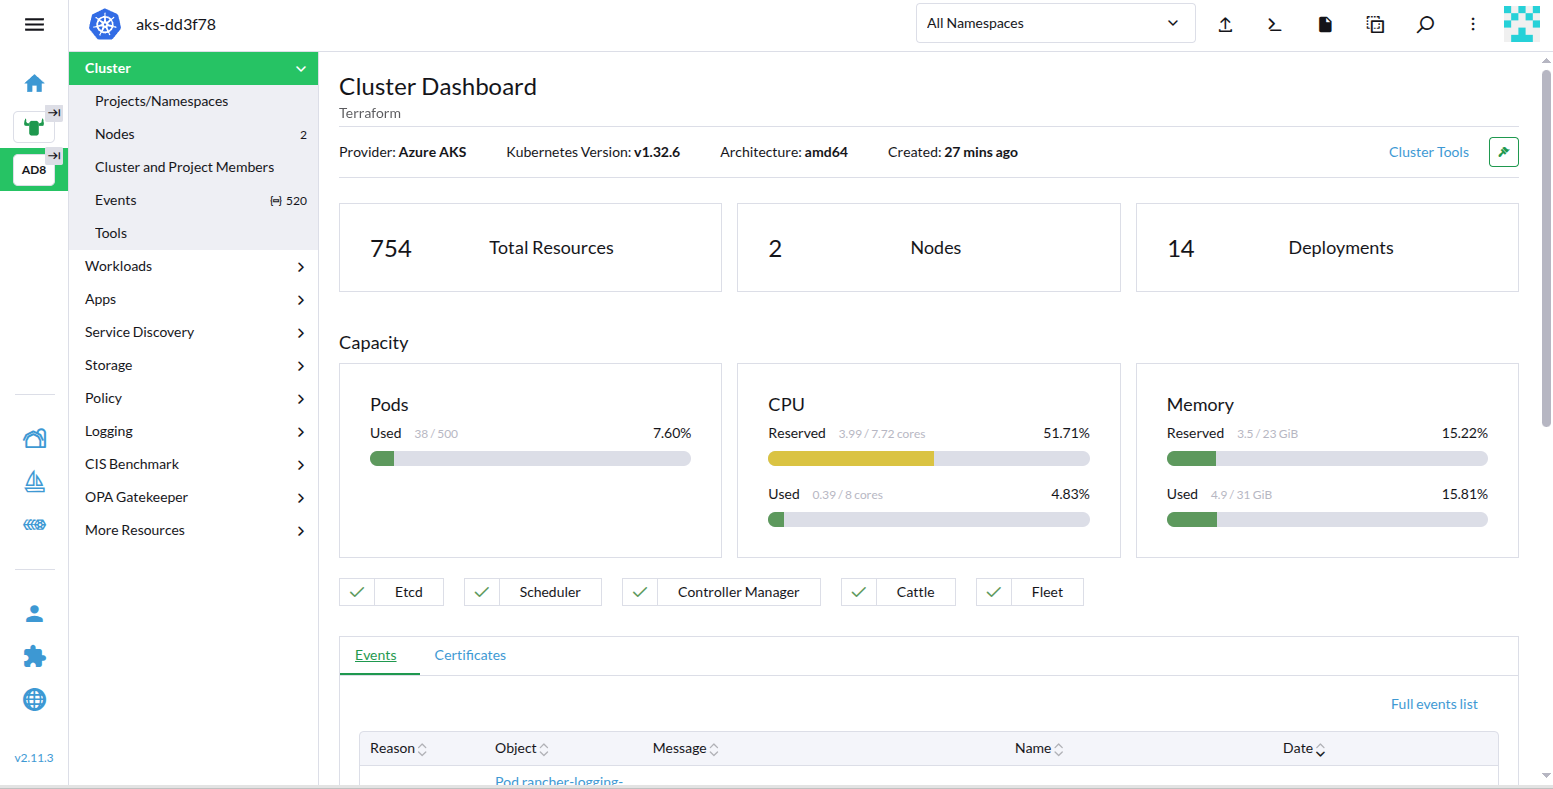
\includegraphics[width=\linewidth]{images/aks-dd3f78.png}
\label{fig:aksdd3f78}
\end{figure}

We then execute the kube-bench job as defined in Chapter 2, and the Benchmark results will become available in the job output:

\begin{figure}[H]
\centering
\caption {Kube-bench Job Output}
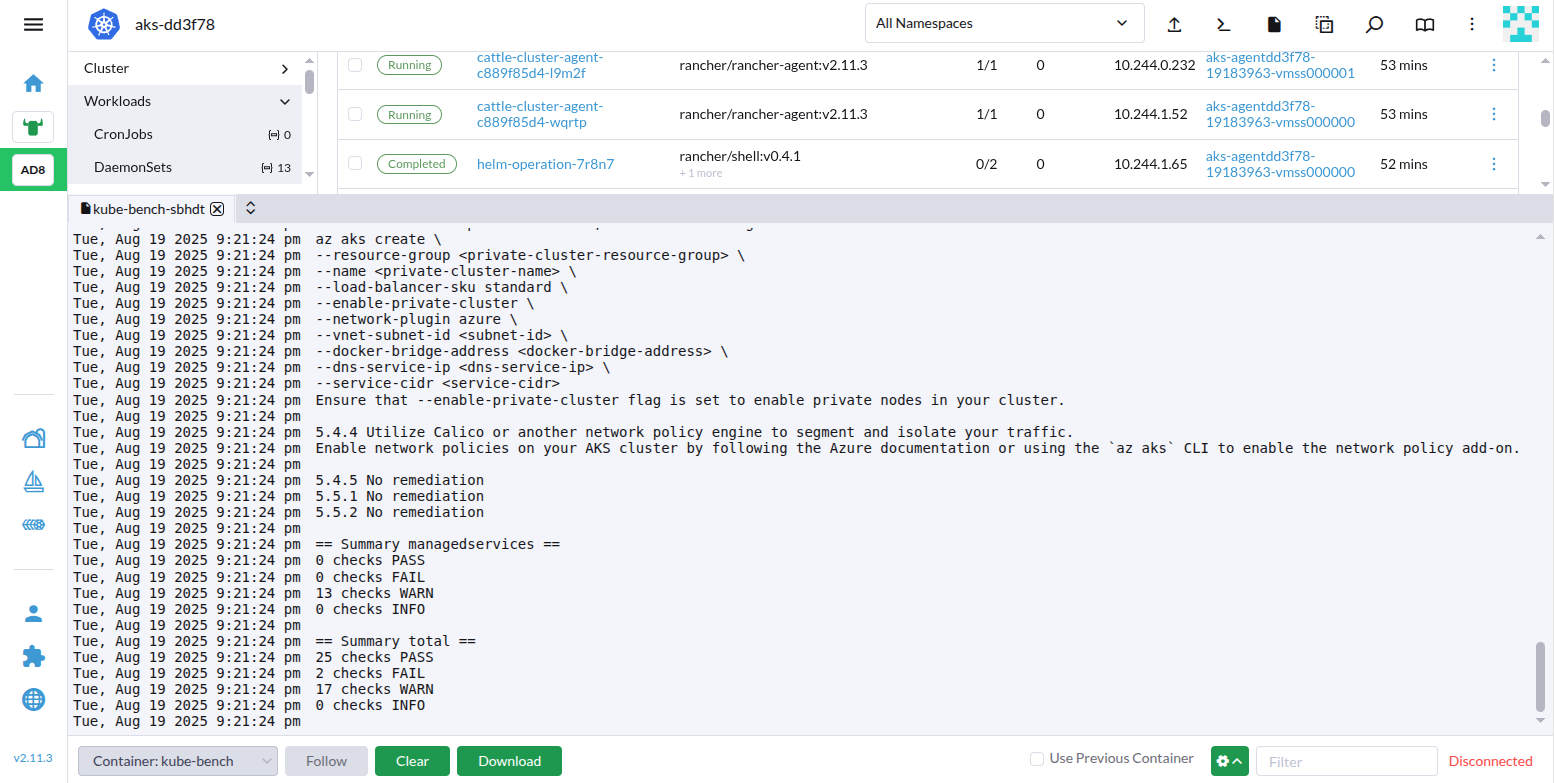
\includegraphics[width=\linewidth]{images/kube-bench-sbhdt.png}
\label{fig:kubesbhdt}
\end{figure}

\pagebreak

\subsection{Benchmarks Findings}

Let's inspect the detailed results from the CIS Benchmark scan, beginning with the worker node security:

\begin{table}[hp]
  \centering
  \caption{CIS Benchmark Scan - Worker Node}
    \begin{tabular}{| l | l | p{11cm} |}
    \hline
    State & ID & Description \\
    \hline\hline
    [PASS] & 3.1.1 & Ensure that the kubeconfig file permissions are set to 644 or more restrictive (Automated) \\
    \hline
    [PASS] & 3.1.2 & Ensure that the kubelet kubeconfig file ownership is set to root:root (Automated) \\
    \hline
    [PASS] & 3.1.3 & Ensure that the azure.json file has permissions set to 644 or more restrictive (Automated) \\
    \hline
    [PASS] & 3.1.4 & Ensure that the azure.json file ownership is set to root:root (Automated) \\
    \hline
    [PASS] & 3.2.1 & Ensure that the --anonymous-auth argument is set to false (Automated) \\
    \hline
    [PASS] & 3.2.2 & Ensure that the --authorization-mode argument is not set to AlwaysAllow (Automated) \\
    \hline
    [PASS] & 3.2.3 & Ensure that the --client-ca-file argument is set as appropriate (Automated) \\
    \hline
    [PASS] & 3.2.4 & Ensure that the --read-only-port is secured (Automated) \\
    \hline
    [PASS] & 3.2.5 & Ensure that the --streaming-connection-idle-timeout argument is not set to 0 (Automated) \\
    \hline
    [PASS] & 3.2.6 & Ensure that the --make-iptables-util-chains argument is set to true (Automated)  \\
    \hline
    [PASS] & 3.2.7 & Ensure that the --eventRecordQPS argument is set to 0 or a level which ensures appropriate event capture (Automated) \\
    \hline
    [PASS] & 3.2.8 & Ensure that the --rotate-certificates argument is not set to false (Automated) \\
    \hline
    [PASS] & 3.2.9 & Ensure that the RotateKubeletServerCertificate argument is set to true (Automated) \\
    \hline
    \end{tabular}%
  \label{tab:aksScanW}%
\end{table}%

As expected, a default installation of a Microsoft AKS cluster will pass all tests for node security, including the important CIS Benchmark test 3.2.1 for anonymous access to the Kubelet server. The CIS Benchmark documentation states the obvious for this test: "You should rely on authentication to authorize access and disallow anonymous requests."\footnote{\textit{CIS (2023)}: CIS AKS Benchmark, 3.2 Kubelet. \cite{cisAks}}

\pagebreak

Next, we'll examine the results for the policies:

\begin{table}[hp]
  \centering
  \caption{CIS Benchmark Scan - Policies}
    \begin{tabular}{| l | l | p{11cm} |}
    \hline
    State & ID & Description \\
    \hline\hline
    [FAIL] & 4.1.1 & Ensure that the cluster-admin role is only used where required (Automated) \\
    \hline
    [PASS] & 4.1.2 & Minimize access to secrets (Automated) \\
    \hline
    [PASS] & 4.1.3 & Minimize wildcard use in Roles and ClusterRoles (Automated) \\
    \hline
    [PASS] & 4.1.4 & Minimize access to create pods (Automated) \\
    \hline
    [PASS] & 4.1.5 & Ensure that default service accounts are not actively used (Automated) \\
    \hline
    [FAIL] & 4.1.6 & Ensure that Service Account Tokens are only mounted where necessary (Automated) \\
    \hline
    [PASS] & 4.2.1 & Minimize the admission of privileged containers (Automated) \\
    \hline
    [PASS] & 4.2.2 & Minimize the admission of containers wishing to share the host process ID namespace (Automated) \\
    \hline
    [PASS] & 4.2.3 & Minimize the admission of containers wishing to share the host IPC namespace (Automated) \\
    \hline
    [PASS] & 4.2.4 & Minimize the admission of containers wishing to share the host network namespace (Automated) \\
    \hline
    [PASS] & 4.2.5 & Minimize the admission of containers with allowPrivilegeEscalation (Automated) \\
    \hline
    [WARN] & 4.4.1 & Ensure latest CNI version is used (Manual) \\
    \hline
    [PASS] & 4.4.2 & Ensure that all Namespaces have Network Policies defined (Automated) \\
    \hline
    [PASS] & 4.5.1 & Prefer using secrets as files over secrets as environment variables (Automated) \\
    \hline
    [WARN] & 4.5.2 & Consider external secret storage (Manual) \\
    \hline
    [WARN] & 4.6.1 & Create administrative boundaries between resources using namespaces (Manual) \\
    \hline
    [WARN] & 4.6.2 & Apply Security Context to Your Pods and Containers (Manual) \\
    \hline
    [PASS] & 4.6.3 & The default namespace should not be used (Automated) \\
    \hline
    \end{tabular}%
  \label{tab:aksScanP}%
\end{table}%

In this section, we encounter two failures due to excessive admin access usage and four warnings concerning network and workload configuration, which should be remedied with the appropriate hardening.

\pagebreak

As the final step, we'll examine the results for managed services:

\begin{table}[hp]
  \centering
  \caption{CIS Benchmark Scan - Managed Services}
    \begin{tabular}{| l | l | p{11cm} |}
    \hline
    State & ID & Description \\
    \hline\hline
    [WARN] & 5.1.1 & Ensure Image Vulnerability Scanning using Microsoft Defender for Cloud (MDC) (Manual) \\
    \hline
    [WARN] & 5.1.2 & Minimize user access to Azure Container Registry (ACR) (Manual) \\
    \hline
    [WARN] & 5.1.3 & Minimize cluster access to read-only for Azure Container Registry (ACR) (Manual) \\
    \hline
    [WARN] & 5.1.4 & Minimize Container Registries to only those approved (Manual) \\
    \hline
    [WARN] & 5.2.1 & Prefer using dedicated AKS Service Accounts (Manual) \\
    \hline
    [WARN] & 5.3.1 & Ensure Kubernetes Secrets are encrypted (Manual) \\
    \hline
    [WARN] & 5.4.1 & Restrict Access to the Control Plane Endpoint (Manual) \\
    \hline
    [WARN] & 5.4.2 & Ensure clusters are created with Private Endpoint Enabled and Public Access Disabled (Manual) \\
    \hline
    [WARN] & 5.4.3 & Ensure clusters are created with Private Nodes (Manual) \\
    \hline
    [WARN] & 5.4.4 & Ensure Network Policy is Enabled and set as appropriate (Manual) \\
    \hline
    [WARN] & 5.4.5 & Encrypt traffic to HTTPS load balancers with TLS certificates (Manual) \\
    \hline
    [WARN] & 5.5.1 & Manage Kubernetes RBAC users with Azure AD (Manual) \\
    \hline
    [WARN] & 5.5.2 & Use Azure RBAC for Kubernetes Authorization (Manual) \\
    \hline
    \end{tabular}%
  \label{tab:aksScanM}%
\end{table}%

All tests in this section are set to warning level, as they mainly deal with systems outside of the Kubernetes cluster, such as the container registry. Also, in the remediations for this section, we can find the recommendation to move from public AKS to private AKS and private endpoints, which would significantly reduce the attack surface.

\subsection{Relevance for NIS2 Article 21}

The identified failures in the scan are both linked to the NIS2 technical implementation guidance 6.3, which generally calls for a "deny-all, permit-by-exception policy."\footnote{See \textit{ENISA (2025)}: Technical Implementation Guidance. \cite{enisaTech}}

Following the principle of least privilege is part of basic cyber hygiene. It should be standard for all critical IT systems that follow established principles for good governance.

To fully comply with the requirements of the NIS2 Directive, additional hardening measures would need to be taken for our cluster by implementing the requirements outlined in the CIS AKS Benchmark results.

\subsection{Implications for DORA compliance}

To support DORA compliance, CIS Security released in April 2025 a mapping for the CIS Controls v8.1 and DORA.\footnote{\textit{CIS (2025)}: CIS Controls v8.1 Mapping to DORA. \cite{cisMapDora}}

The mappings seem to be very similar to the mappings for the NIS2 Directive; a detailed analysis could be the subject of a further paper, with a similar outcome likely.

\subsection{Overall Compliance and Risk Mitigation}

We have seen Microsoft's Azure Kubernetes Engine partly pass the AKS CIS Benchmark v1.7 and might need additional hardening for full compliance. The other major hosted versions of Kubernetes, Google's Kubernetes Engine (GKE) and Amazon's Elastic Kubernetes Service (EKS), also offer CIS compliance and remediation guidance to their customers.

On-premise Kubernetes distributions, such as SUSE's Rancher or Red Hat's OpenShift, offer optional CIS compliance and hardening, too. 

Ensuring that an IT system, such as a Kubernetes cluster, scores a passing grade on the CIS Benchmarks supports basic cyber hygiene and should be part of any IT Security Policy.

\subsection{Outlook}

Article 21 of the NIS 2 Directive outlines the cybersecurity risk-management measures essential entities must implement to protect their networks and information systems. These measures are designed to prevent and minimize the impact of cyber incidents on both the entities and their customers. It outlines critical cybersecurity practices that every business under the NIS2 regulations must have in place. 

One mandatory cybersecurity measure under Article 21 is basic cyber hygiene practices and training, as described in paragraph 2(g).

This requirement is where NIS2, the CIS Controls, and the CIS Benchmarks intersect. The CIS Benchmarks outline and implement procedures to fulfill CIS Control 04, Secure Configuration, a crucial requirement for basic cyber hygiene and part of any IT Security Policy.

As we've seen above, CIS Benchmarks can be used to enforce good security practices by automatically checking for deviations and issues. CIS Benchmarks can also recommend the necessary steps for remediation.

We can conclude that a passing result for the appropriate CIS Benchmark can serve as a good indicator of whether the Kubernetes cluster is NIS2 compliant.

Passing the CIS Benchmark alone is not a sufficient indicator, though, as the NIS2 Directive includes many more aspects than the basic cyber hygiene outlined in Article 21; however, failing the CIS Benchmark, as in our case, will be a clear indicator that the Kubernetes cluster as part of the IT platform is not NIS2 compliant.

NIS2 is a legal framework, and compliance will be mandatory for European critical entities, ensuring widespread adoption. Unlike the CISecurity or ISO 27001 frameworks, adherence to the NIS2 Directive's requirements is not optional for entities classified as important or particularly important; it will be mandated by law.

In addition to Article 21, the NIS2 Directive also contains Article 23, which outlines the requirements for EU-wide incident reporting. Article 23 defines what constitutes an incident, the mandatory reports, and the content required in these reports. With pan-European reporting of cyber attacks, a coordinated response should become much more manageable.


%
%	Fazit
%

\pagebreak
\section{Summary}

\onehalfspacing

The Center of Internet Security offers benchmarks against which to test a Kubernetes cluster. Rancher has integrated CIS scans and can mitigate the findings.

The CIS Benchmarks cover CIS Controls v8 4.1, which corresponds to Article 21 2(g) of the Network and Information Systems Directive II.

As NIS2 matures, we hope to see more formal mappings with CIS Controls v8 and its Implementation Groups to ease practical implementation.

For now, we can conclude that the CIS Benchmarks will help enterprises to fulfill and monitor the requirements for basic cyber hygiene as outlined in Article 21 2(g).

Upcoming legislation, such as the KRITIS-DachG ("Gesetz zur Umsetzung der Richtlinie (EU) 2022/2557 und zur Stärkung der Resilienz von Betreibern kritischer Anlagen"), will further strengthen the security posture of IT systems in the EU.

Regardless of future developments, governance, risk management, and regulatory compliance will remain critical topics in Enterprise IT, and the CIS Benchmarks are a good tool for monitoring IT systems compliance.

The Terraform plan files for the downstream clusters used in this paper are on my \href{https://github.com/chfrank-cgn/Rancher}{GitHub}.

Happy Ranching!


%
%	Tools (Sopron)
%

\pagebreak
\section{Tools}

\onehalfspacing

In addition to the documented references, these tools were used in creating this paper:

\begin{itemize}
    \item \href{http://www.overleaf.com}{Overleaf} to write the LaTeX source code
    \item \href{https://github.com/chfrank-cgn}{GitHub} for backup and version control
    \item Anthropic's \href{https://www.anthropic.com/claude}{Claude} for research
    \item \href{https://app.grammarly.com/}{Grammarly} for spellcheck and style
\end{itemize}


% Literaturverzeichnis
\cleardoublepage
\raggedright
\bibliographystyle{IEEEtranS}	% ieeetran verwenden, damit auch URLs angezeigt werden
\bibliography{seminar-lit}

\cleardoublepage
\justify
%
%	Ehrenwoertliche Erklaerung
%

\pagebreak

\pagenumbering{gobble} % Keine Seitenzahlen mehr
\onehalfspacing

%-----------------------------------
% Ehrenwoertliche Erklärung
%-----------------------------------
\section*{Declaration in lieu of oath}

\par\medskip

With this, I declare that I produced the submitted paper without any other party's assistance and without using any unauthorized aids. In particular, I have marked all passages reproduced verbatim or near-verbatim from publications as quotations. Also, I declare that the submitted print version of this thesis is identical to its digital version. Further, I have never introduced this thesis to any examination board in its present form or any other similar version. I herewith agree that you may publish this thesis. I herewith consent to you uploading this thesis to an external contractor's server to submit it to the contractor's plagiarism detection systems. Uploading this thesis to send it to plagiarism detection systems is not a form of publication.

\par\medskip
\par\medskip

\vspace{5cm}

\begin{table}[H]
	\begin{tabular*}{\textwidth}{c @{\extracolsep{\fill}} ccccc}
		Cologne, \the\month/\the\day/\the\year \\
		\rule[0.5ex]{12em}{0.55pt} & \rule[0.5ex]{12em}{0.55pt} \\
		(Location, Date) & (Signature)
	\end{tabular*}
\end{table}


\end{document}
